\chapter{CONDICIONES GENERALES Y CONDICIONES LIMITANTES.} %(((

\begin{enumerate}
	\item De acuerdo con las facturas proporcionadas, los equipos son propiedad de BBVA Leasing México, S.A. de C.V.
	\item No se incluyeron inventarios de ningún tipo, ni cualquier otro activo circulante o intangible, así como tampoco permisos, derechos, cuotas de contratación, etc., necesarios para la obtención de los diversos servicios de tipo operativo tales como: agua, energía eléctrica y similares, etc., así como tampoco el impuesto de valor agregado.
	\item El tipo de cambio empleado para el presente avalúo se toma a la fecha del \fechaInforme, de acuerdo con los datos publicados en la página del Banco de México, la paridad empleada fue de \$18.7822 MXN por dólar americano y de \$20.2079 MXN por euro.
	\item La estimación de los valores se considera de acuerdo con el estado y condición observados.
	\item No se proporcionaron bitácoras de mantenimiento, ya que los equipos están fuera de operación.
	\item No se tomaron en cuenta descuentos especiales por parte de los proveedores, se consideran puestos en el país y no se incluye el impuesto al valor agregado (IVA) para los valores de cotización reportados.
	\item Se consideró la información proporcionada y los datos de placa para establecer la edad de los bienes de los equipos que la contenían.
	\item No nos hacemos responsables por vicios ocultos o fallos no detectados durante la inspección o daños en el proceso de traslado y desinstalación.
\end{enumerate}

\section{NOTAS IMPORTANTES.} % (((
\begin{enumerate}
\setcounter{enumi}{8}
\item El análisis del presente servicio fue limitado, ya que no se permitió la toma de fotografías ni de datos adicionales como la capacidad y fichas técnicas. Por lo tanto únicamente se considera como descripción general lo observado en la identificación de los equipos e investigación realizada por COFINSA para la localización de los proveedores y  comparativos de equipos similares de la misma procedencia.
\item Para los activos 1, 2, 3, 4, 5, 6, 7, 8, 9, 10, 11, 23, 24, 25, 26, 27, 28, 29, descritas en el inventario de maquinaria y equipo se verificaron físicamente, sin embargo, no pudo verificarse ni su estado de conservación y placa de datos.
\item Para el activo 4.1-9, por las instrucciones de BBVA Leasing, únicamente se valúa la línea de secado de aire caliente marca Jinan Dayi, ``Extrusión Food Machinery'', modelo SHX-IV, no. serie 192950027, no. económico 2452200, de acuerdo con inventario proporcionado. Los equipos faltantes son: Z type Bucket y 5M Cooling Mayor.
\item Para los activos 1, 2, 3, 4, 5, 6, 7, 8, 9, 10, 11, 23, 24, 25, 26, 27, 28, 29, 39, 40, 41, 42, 43, 44, 45, 46, 47, 48, 49, 50, 51,  descritas en el inventario de maquinaria y equipo los cuales no se cuenta con fotografías de la placa de datos,  se considera como fecha de fabricación,  el año de la factura la cual fue proporcionada por BBVA Leasing.
\item Para los activos 44, 45, 46, 47, 48, 49, 50, 51,  descritas en el inventario de maquinaria y equipo,  al momento de la visita se tomaron los datos y las cantidades de los elevadores de cangilones con los cuales podía operar los equipos,  mismos que se describe la cantidad en cada una de las partidas antes mencionadas.
\item La información técnica y capacidades obtenidas de la documentación proporcionada por BBVA Leasing, de los equipos descritos en el inventario de maquinaria y equipo, se considera veraz y correcta.
\item No hubo personal asignado por parte de la empresa que proporcionara bitácoras de mantenimiento o histograma de reparaciones mayores de los equipos por lo que no fue posible verificar su estado de conservación.
\item De acuerdo con investigación realizada por COFINSA, las máquinas seleccionadoras, de acuerdo al proveedor pueden ser utilizadas para arroz u otros cereales, por lo que no son adecuadas para las nueces.
\item Con los efectos de reporte se indica a continuación Tabla de Parámetros, donde cada sujeto (M\&E), se compara el monto cotizado contra el monto indicado de factura, así como las variaciones entre uno y otro concepto. 
\end{enumerate}
\begin{figure}[hbtp!]
	\centering
	\caption{Reporte General Comparativo (Cotización VS Facturación.)}
	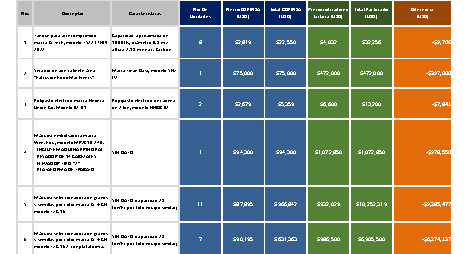
\includegraphics[width=  \linewidth,page=1]{../0.imagenes/CAP_3/cap_3}
	\label{fig:comparartivo}
\end{figure}
\newpage
\begin{figure}[hbtp!]
	\centering
	\includegraphics[width=  \linewidth,page=2]{../0.imagenes/CAP_3/cap_3}
\end{figure}
% )))

% )))
